\documentclass[12pt,addpoints,answers]{guia}
\grado{2$^\circ$ de Secundaria}
\cicloescolar{2022-2023}
\materia{Física 2}
\guia{2}
\unidad{3}
\title{Energía cinética}
%\unidad{3}
\title{El título de la guía}
\aprendizajes{\item Analiza la energía mecánica (cinética y potencial) y describe casos donde se conserva.
    }
\author{JC Melchor Pinto}
\begin{document}
\pagestyle{headandfoot}

\INFO
%\printanswers
\begin{opening}[Energía del movimiento]{
        \begin{minipage}{0.35\textwidth}
            \begin{figure}[H]
                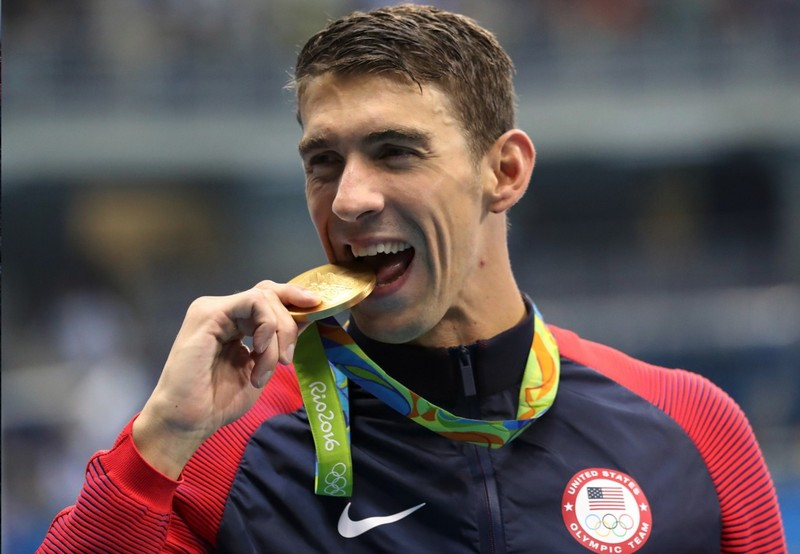
\includegraphics[width=\linewidth]{../images/michael_phelps.jpg}
            \end{figure}
        \end{minipage}\hfill
        \begin{minipage}{0.6\textwidth}
            Si has andado en bicicleta, jugado futbol o competido en una carrera, sabrás
            que después del ejercicio te sientes cansado. ¿Sabías que Michel Phelps
            (1985), nadador estadounidense que ha ganado 28 medallas olímpicas, para
            entrenar comía lo mismo que cinco adultos? Es un hecho que para llevar a
            cabo un esfuerzo físico se requiere energía, y por eso, después de ejercitarnos, sentimos hambre.
            Con lo anterior queremos decir que el movimiento
            está relacionado con la energía. La energía que posee un cuerpo debido a
            su movimiento se conoce como \textbf{energía cinética} (del griego kinetos: que se
            mueve). Si te has golpeado con un balón de futbol o te has golpeado un dedo
            del pie contra un mueble mientras caminas, entonces has sentido los efectos de
            la energía cinética.\\
        \end{minipage}
        La \textbf{energ\'ia cin\'etica} de un cuerpo en movimiento depende de
        dos variables o magnitudes f\'isicas: su masa (m) y su rapidez (v). La ecuaci\'on
        que relaciona ambas variables y define a la energ\'ia cin\'etica ($E_C$) es:

        \begin{equation}\label{cinetica}
            E_c=\frac{1}{2}mv^2
        \end{equation}

        Las unidades de la energ\'ia cin\'etica, derivadas a partir de su ecuaci\'on, son las
        de masa por las de rapidez al cuadrado: kg m$^2$/s$^2$, que corresponden a las
        unidades de la energ\'ia en el SI (Sistema Internacional); es decir, al joule (J). Como sabes, la unidad de fuerza es el
        newton (N), y 1 N equivale a 1 kg m/s$^2$, de manera que: \( 1 J = 1 kg m^2/s^2 = 1 Nm \)

    }
\end{opening}
\begin{questions}
    \include*{../questions/question003}
    \fullwidth{\begin{boxG}
            La ecuación (\ref{cinetica}) de la energía cinética  tiene una variable elevada al cuadrado: la velocidad. En la mayoría de los casos se usa como
            dato una velocidad positiva. Sin embargo, recuerde a los alumnos que cualquier
            cantidad elevada al cuadrado siempre tendrá un valor positivo. Así mismo, es importante que consideren el cuadrado también para las unidades pues, de omitirlo,
            no sería posible hallar las unidades correspondientes a la energía.
        \end{boxG}}
    \include*{../questions/question006}
    \newpage
    \fullwidth{\begin{boxG}
            La ecuación (\ref{cinetica}) requiere que las unidades de la velocidad sean expresadas en m/s. Si la velocidad se encuentra en km/h se recomienda convertir dicha variable para ser consistentes con las unidades de energía, Joules (J).
        \end{boxG}}
    \include*{../questions/question004}
    \include*{../questions/question008}
    \newpage
    \include*{../questions/question009}
    \newpage
    \fullwidth{\begin{boxG}
            De manera general, la ecuación (\ref{cinetica}) puede ser utilizada para calcular cualquiera de las variables, incluyendo la masa del objeto y su velocidad. Para ello, deberas preparar la ecuación despejando la variable de tu interés.
            \begin{center}
                $E_c=\frac{1}{2}mv^2$ \qquad   $m=\dfrac{2E_c}{v^2}$ \qquad  $v=\sqrt{\dfrac{2E_c}{m}}$
            \end{center}
        \end{boxG}}
    \include*{../questions/question007}
    \include*{../questions/question005}
    \include*{../questions/question010}

\end{questions}

%\vfill
%\puntuacion

\end{document}